\documentclass[10pt]{beamer}
\usepackage[magyar]{babel}
\usepackage[utf8]{inputenc}
\usepackage{t1enc}
\usepackage{wrapfig}
\usetheme[pageofpages=/,alternativetitlepage=true,]{Torino}
\usecolortheme{freewilly}
\usepackage{mathtools}

\author{Olar Alex}
\title{Az Einstein-egyenletek Schwarzschild-megoldása}
\institute{Eötvös Loránd Tudományegyetem \\ \scriptsize{Fizika BSc III.}}
\date{A klasszikus térelmélet elemei szeminárium, 2017. december}


\begin{document}
\begin{frame}[t,plain]
\titlepage
\end{frame}

\begin{frame}[t]{Vázlat}
\begin{itemize}
\item Történeti bevezető
\item A probléma megfogalmazása
\item Számolás
\item Összefoglalás
\item Hivatkozások
\end{itemize}
\end{frame}

\begin{frame}[t]{Történeti bevezető}
\begin{wrapfigure}{r}{0.4\textwidth}
\caption{Karl Schwarzschild}
\begin{center}
	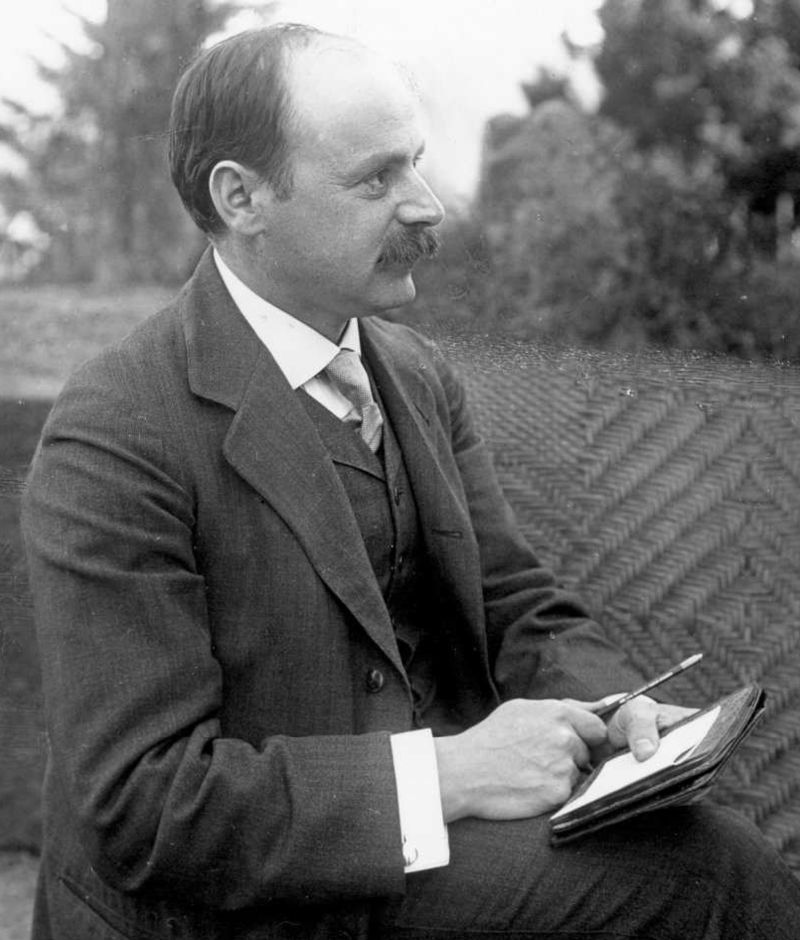
\includegraphics[width=0.35\textwidth]{karl.jpg}
\end{center}
\end{wrapfigure}
\par Karl Schwarzschild (1873 - 1916) német fizikus volt. Ő állt elő az Einstein-egyenletek első egzakt megoldásával, méghozzá a
gömbszimmetrikus, M tömegű, R sugarú, nyugalomban lévő testre vonatkozólag oldotta meg a téregyenleteket. Mindezt az első
világháború alatt, a frontszolgálat közben sikerült kiviteleznie.
\end{frame}

\begin{frame}[t]{A probléma megfogalmazása}
\texttt{Milyen metrikájú a téridő egy gömbszimmetrikus, R sugarú, M tömegű, sztatikus testen kívül? }
\vspace{3mm}
\par A gömbkoordinátákkal kifejezve az ívemelem négyzet Minkowski-térben a következő alakot ölti (c = 1):
\begin{equation*}
ds^{2} = dt^{2} - dr^{2} -r^{2}d\vartheta^{2} - r^{2}sin^{2}\vartheta d\varphi^{2}
\end{equation*}
\par Azaz a síkban vett metrikus tenzor a következő:
$$
\eta = \begin{pmatrix}
1& & &  \\
& -1& &  \\
& & -r^{2}&  \\
& & & -r^{2}sin^{2}\vartheta
\end{pmatrix}
$$
\par Ahol figyelni kell arra, hogy a szignatúra (+,-,-,-) legyen.
\end{frame}

\begin{frame}[t]{A probléma megfogalmazása}
Most ezt kellene a megfelelő módon módosítani:
$$
g = \begin{pmatrix}
U& & &  \\
& -V& &  \\
& & -Wr^{2}&  \\
& & & -Xr^{2}sin^{2}\vartheta
\end{pmatrix}
$$
\par Ahol kezdetben U,V,W,X függvények az $(r,\vartheta,\varphi,t)$ változók általános függvényei. Felhasználva a probléma
speciális tulajdonságait:
\begin{itemize}
\item gömbszimmetria alatt azt lehet érteni, hogy a metrikus tenzorban kiemelt U,V,W,X függvények nem függnek $(\vartheta, 
\varphi)$ változóktól, tehát csakis az $r$ mennyiség függvénye, valamint az.
\item sztatikus problémáról van szó, így feltehető, hogy az időfüggés elhagyható
\end{itemize}
\end{frame}

\begin{frame}[t]{A probléma megfogalmazása}
\begin{itemize}
\item a vákuum-megoldás keresése közben, az objektumon kívül az energia-impulzus tenzor azonosan nulla : $T_{kl}\equiv 0$
\item Schwarzzschild eredetileg nem így írta fel az egyenleteket. Ő módosított gömbipolár-koordinátákat vezetett be
\begin{gather*}
x^{1} = \frac{r^{3}}{2} \quad x^{2} = -cos\vartheta \quad x^{3} = \varphi \quad x^{4} = t
\end{gather*}
\begin{itemize}
\item az ebből $ds^{2}$-re kapott egyenletből származtatható a mostani esetre vonatkoztatva, hogy elegendő a $W = X = 1$ esetet
vizsgálni
\end{itemize}
\item azaz az ívelemnégyzetre a következő kifejezést kapjuk
 $$ ds^{2} = U(r)dt^{2} - V(r)dr^{2} -r^{2}d\vartheta^{2} -r^{2}sin^{2}\vartheta d\varphi^{2} $$
\end{itemize}
\end{frame}

\begin{frame}[t]{A probléma megfogalmazása}
\par Ahol a metrikus  tenzor inverze a következő (az inverz jelölése ugyanaz):
$$
g = G = \begin{pmatrix}
\frac{1}{U}& & &  \\
& -\frac{1}{V}& &  \\
& & -\frac{1}{r^{2}}&  \\
& & & -\frac{1}{r^{2}sin^{2}\vartheta}
\end{pmatrix}
$$
\vspace{4mm}
\par Hiszen a $g_{kl}g^{kl} = 4$ egyenlet teljesül, ahol a latin ábécé betűivel nullától háromig lévő indexeket jelölöm, míg
a görög ábécé betűivel az egytől háromig terjedőeket, tehát $k \in \{0,1,2,3\}$, $\alpha \in \{1,2,3\}$
\vfill
\par A továbbiakban is mindig ezt a konvenciót használja a prezentáció.
\end{frame}

\begin{frame}[t]{A probléma megfogalmazása}
A megoldandó probléma tehát az Einstein-egyenletek (a kozmológiai állandó zérus) megoldása egy gömbszimmetrikus, sztatikus objektumon kívül.
\begin{equation*}
E_{kl} = G_{kl} = R_{kl} - \frac{R}{2}g_{kl} = \frac{8\pi G}{c^{4}}T_{kl} = 0
\end{equation*}
\par Amely egyenletben $c^{4}$ tag csak hagyománytiszteletből szerepel (c = 1). $R_{kl}$ a Ricci-tenzor, amit a Riemann-féle 
görbületi tenzorból származtatható (első és harmadik index összeejtésével például), $R$ pedig a Ricci-skalár mennyiség, amely
a Ricci-tenzor spurja.
\vspace{3mm}
\par $E_{kl}$ vagy az irodalomban gyakrabban $G_{kl}$ az Einstein-tenzor, $G$ pedig a Newton féle gravitációs 
konstans.
\end{frame}

\begin{frame}[t]{A probléma megfogalmazása}
\par Ahol a metrikus  tenzor inverze a következő (az inverz jelölése ugyanaz):
$$
g = G = \begin{pmatrix}
\frac{1}{U}& & &  \\
& -\frac{1}{V}& &  \\
& & -\frac{1}{r^{2}}&  \\
& & & -\frac{1}{r^{2}sin^{2}\vartheta}
\end{pmatrix}
$$
\vspace{4mm}
\par Hiszen a $g_{kl}g^{kl} = 4$ egyenlet teljesül, ahol a latin ábécé betűivel nullától háromig lévő indexeket jelölöm, míg
a görög ábécé betűivel az egytől háromig terjedőeket, tehát $k \in \{0,1,2,3\}$, $\alpha \in \{1,2,3\}$
\vfill
\par A továbbiakban is mindig ezt a konvenciót használja a prezentáció.
\end{frame}

\begin{frame}[t]{A probléma megfogalmazása}
\begin{itemize}
\item Riemann - tenzor
\begin{itemize}
\item $R^{k}_{lmp} = \partial_{m}\Gamma_{lp}^{k} - \partial_{p}\Gamma_{lm}^{k} + \Gamma_{lp}^{q}\Gamma_{qm}^{k} - \Gamma_{lm}^{q}\Gamma_{qp}^{k}$
\end{itemize}
\item Ricci - tenzor
\begin{itemize}
\item $R^{s}_{lsp} = R_{lp} = \partial_{s}\Gamma_{lp}^{s} - \partial_{p}\Gamma_{ls}^{s} + \Gamma_{lp}^{q}\Gamma_{qs}^{s} - \Gamma_{ls}^{q}\Gamma_{qp}^{s}$
\end{itemize}
\item Ricci - skalár
\begin{itemize}
\item $g^{kl}R_{kl} = R_{k}^{k}$
\end{itemize}
\end{itemize}
\par Ezeken felül még ki kell használni, hogy a Christoffel-szimbólumokat a metrikus tenzorból kapható.
\begin{equation*}
\Gamma_{lm}^{k} = \frac{1}{2}g^{ks}(\partial_{m}g_{sl} + \partial_{l}g_{sm} - \partial_{s}g_{lm})
\end{equation*}
\par A későbbiekben felhasználásra kerül, hogy a $\Gamma$ mennyiségek az alsó két indexükben torzió mentesek, azaz 
szimmetrikusak.
\end{frame}

\begin{frame}[t]{Számolás}
\texttt{Meg kell határozni a $\Gamma$ mennyiségek (nem tenzor) minden komponensét.} Ez rengeteg számítást igényelne
(64 elem, ha nem vesszük a torziómentességet), tehát vagy gondolkozunk vagy használunk egy szimbolikus nyelvet, amely képes
ilyen számolásokra (Wolfram Mathematica).
\par A következőket kell figyelembe venni:
\begin{itemize}
\item torziómentesség $\Gamma_{ik}^{l} = \Gamma_{ki}^{l}$
\item minden $\partial_{0}$ deriváltja a metrikus tenzornak azonosan nulla $\partial_{0}g_{ik}\equiv 0$
\item a metrikus tenzor nem diagonális elemei azonosan nullát adnak
\end{itemize}
\vfill
\par Ezen információk birtokában...
\end{frame}

\begin{frame}[t]{Számolás}
$$k = 0 \rightarrow \Gamma_{lm}^{0} = \frac{1}{2}g^{0s}(\partial_{m}g_{sl} + \partial_{l}g_{sm} - \partial_{s}g_{lm})$$
\par Ezután, mivel a metrikus tenzor diagonális csak $s = 0$ esetben nem azonosan nulla megoldást kapunk.
\begin{gather*}
\Gamma_{lm}^{0} = \frac{1}{2}g^{00}(\partial_{m}g_{0l} + \partial_{l}g_{0m} - \partial_{0}g_{lm}) \rightarrow \partial_{0}g_{lm} \equiv 0 \\
l = 0 \rightarrow \Gamma_{0m}^{0} = \frac{1}{2}g^{00}(\partial_{m}g_{00} + \partial_{0}g_{0m}) \partial_{0}g_{0m} \equiv 0 \\
\Gamma_{0m}^{0} = \delta_{m}^{1}\frac{1}{2}g^{00}\partial_{1}g_{00} = \delta_{m}^{1}\frac{1}{2}\frac{1}{U}\partial_{r}U
\end{gather*}
\par Azaz az első két nem nulla elem 
\begin{gather*}
\Gamma_{01}^{0} = \Gamma_{10}^{0} = \frac{U'}{2U} \\
\Gamma_{ij}^{0} \equiv 0 \quad amikor \quad \{i,j\} \neq \{0,1\} \quad vagy \quad \{1,0\}
\end{gather*}
\end{frame}

\begin{frame}[t]{Számolás}
$$k = 1 \rightarrow \Gamma_{lm}^{1} = \frac{1}{2}g^{1s}(\partial_{m}g_{sl} + \partial_{l}g_{sm} - \partial_{s}g_{lm})$$
\par Ezután, mivel a metrikus tenzor diagonális csak $s = 1$ esetben nem azonosan nulla megoldást kapunk.
\begin{gather*}
\Gamma_{lm}^{1} = \frac{1}{2}g^{11}(\partial_{m}g_{1l} + \partial_{l}g_{1m} - \partial_{1}g_{lm}) \\
l = 0 \rightarrow \Gamma_{0m}^{1} = -\frac{1}{2}g^{11}(\partial_{1}g_{0m}) = 
-\delta_{0}^{m}\frac{1}{2}g^{11}\partial_{m}g_{00} \\
l = 1 \rightarrow \Gamma_{1m}^{1} = \frac{1}{2}g^{11}(\partial_{m}g_{11} + \partial_{1}g_{1m} - \partial_{1}g_{1m}) = \delta_{1}^{m}
\frac{1}{2}g^{11}\partial_{m}g_{11} \\
l = 2 \quad \Gamma_{2m}^{1} = \frac{1}{2}g^{11}(\partial_{m}g_{12} + \partial_{2}g_{1m} - \partial_{1}g_{2m}) \rightarrow
-\delta_{2}^{m}\frac{1}{2}g^{11}\partial_{m}g_{22} \\
l = 3 \quad \Gamma_{3m}^{1} = \frac{1}{2}g^{11}(\partial_{m}g_{13} + \partial_{3}g_{1m} - \partial_{1}g_{3m}) \rightarrow
-\delta_{3}^{m}\frac{1}{2}g^{11}\partial_{m}g_{33}\\
 \Gamma_{00}^{1} = \frac{U'}{2V} \quad \Gamma_{11}^{1} = \frac{V'}{2V} \quad \Gamma_{22}^{1} = -\frac{r}{V} \quad \Gamma_{33}^{1}=-\frac{rsin^{2}\vartheta}{V} \\
\end{gather*}
\end{frame}

\begin{frame}[t]{Számolás}
$$k = 2 \rightarrow \Gamma_{lm}^{2} = \frac{1}{2}g^{2s}(\partial_{m}g_{sl} + \partial_{l}g_{sm} - \partial_{s}g_{lm})$$
\par Ezután $s = 2$ 
\begin{gather*}
\Gamma_{lm}^{2} = \frac{1}{2}g^{11}(\partial_{m}g_{2l} + \partial_{l}g_{2m} - \partial_{2}g_{lm}) \\
l = 2 \rightarrow \Gamma_{2m}^{2} = \frac{1}{2}g^{22}(\partial_{m}g_{22}) = 
-\delta_{1}^{m}\frac{1}{2}g^{22}\partial_{m}g_{00}\\
l = 1 \rightarrow \Gamma_{1m}^{1} = \frac{1}{2}g^{11}(\partial_{m}g_{11} + \partial_{1}g_{1m} - \partial_{1}g_{1m}) = \delta_{m}^{1}
\frac{1}{2}g^{11}\partial_{1}g_{11} \\
\Gamma_{21}^{2} = \Gamma_{12}^{2} = \frac{1}{r}
\end{gather*}
\par Az első képleten látható, hogy a többi esetben csak az utolsó tag marad meg ahol 
$\partial_{2} = \partial_{\vartheta}$ - tól csak $g_{33}$ függ, tehát:
\begin{gather*}
l = 3 \quad m = 3 \rightarrow \Gamma_{33}^{2} = \frac{1}{2}g^{22}(\partial_{3}g_{33}) = -sin\vartheta cos\vartheta \\
\end{gather*}
\end{frame}

\begin{frame}[t]{Számolás}
$$k = 3 \rightarrow \Gamma_{lm}^{3} = \frac{1}{2}g^{3s}(\partial_{m}g_{sl} + \partial_{l}g_{sm} - \partial_{s}g_{lm})$$
\par Ezután $s = 3$ 
\begin{gather*}
\Gamma_{lm}^{3} = \frac{1}{2}g^{33}(\partial_{m}g_{3l} + \partial_{l}g_{3m} - \partial_{3}g_{lm}) \\
l = 3 \rightarrow \Gamma_{3m}^{3} = \frac{1}{2}g^{33}(\partial_{m}g_{33}) \rightarrow 
\frac{1}{2}g^{33}\partial_{1}g_{33} \quad vagy \quad \frac{1}{2}g^{33}\partial_{2}g_{33}\\
\Gamma_{31}^{3} = \Gamma_{13}^{3} = \frac{1}{r} \\
\Gamma_{32}^{3} = \Gamma_{23}^{3} = \frac{1}{tg\vartheta} \\
\end{gather*}
A többi tag mind nulla, mivel az első egyenletre visszanézve látható, hogy $\partial_{3}$-tól egyik tag sem függhet, valamint
a többi tag pedig figyelembe lett véve.
\end{frame}

\begin{frame}[t]{Számolás}
\texttt{Szerencsére 'csak' ennyi tag nem nulla, mint ahogy az látható volt, ezeket összefoglalva:}
\begin{gather*}
\Gamma_{00}^{1} = \frac{U'}{2V} \quad \quad \Gamma_{11}^{1} = \frac{V'}{2V} \\
\Gamma_{22}^{1} = -\frac{r}{V} \quad \quad \Gamma_{33}^{1}=-\frac{rsin^{2}\vartheta}{V} \\
\Gamma_{21}^{2} = \Gamma_{12}^{2} = \frac{1}{r} \quad \Gamma_{33}^{2} = -sin\vartheta cos\vartheta \\
\Gamma_{31}^{3} = \Gamma_{13}^{3} = \frac{1}{r} \quad \quad \Gamma_{32}^{3} = \Gamma_{23}^{3} = \frac{1}{tg\vartheta} \\
\Gamma_{01}^{0} = \Gamma_{10}^{0} = \frac{U'}{2U} \\
\end{gather*}
\par Ez 13 tag, most ezeknek a segítségével kell kiszámolni a Ricci-tenzort.
\end{frame}

\begin{frame}[t]{Számolás}
Korábban láttuk $$R^{s}_{lsp} = R_{lp} = \partial_{s}\Gamma_{lp}^{s} - \partial_{p}\Gamma_{ls}^{s} + \Gamma_{lp}^{q}\Gamma_{qs}^{s} - \Gamma_{ls}^{q}\Gamma_{qp}^{s}$$
Most $l \neq p$ esetek, off-diagonális esetek:
\begin{gather*}
l = 0 \quad p = \alpha \rightarrow R_{0\alpha} = \partial_{s}\Gamma_{0\alpha}^{s} - \partial_{\alpha}\Gamma_{0s}^{s} + \Gamma_{0\alpha}^{q}\Gamma_{qs}^{s} - \Gamma_{0s}^{q}\Gamma_{q\alpha}^{s}
\rightarrow \partial_{\alpha}\Gamma_{0s}^{s} \equiv 0 \\
R_{0\alpha} = \partial_{1}\Gamma_{0\alpha}^{1} + \partial_{2}\Gamma_{0\alpha}^{2} + \Gamma_{0\alpha}^{1}\Gamma_{11}^{1} + 
\Gamma_{0\alpha}^{1}\Gamma_{12}^{2} + \Gamma_{0\alpha}^{1}\Gamma_{10}^{0} + \Gamma_{0\alpha}^{2}\Gamma_{23}^{3} + 
\Gamma_{0\alpha}^{1}\Gamma_{13}^{3} + \\
 - \Gamma_{00}^{1}\Gamma_{1\alpha}^{0} - \Gamma_{01}^{1}\Gamma_{0\alpha}^{1} \\
R_{0\alpha} = \Gamma_{0\alpha}^{1}(\Gamma_{11}^{1} + \Gamma_{12}^{2} + \Gamma_{13}^{3}) + \partial_{1}\Gamma_{0\alpha}^{1}
- \Gamma_{00}^{1}\Gamma_{1\alpha}^{0} \equiv 0
\end{gather*}
\par Az utolsó ekvivalencia azért helyes, mert $\alpha = 0$ eseten kívül, ami nem megengedett, a szereplő tagok mind zérusok. Továbbá:
$$R_{00} = \Gamma_{00}^{1}(\Gamma_{11}^{1} + \Gamma_{12}^{2} + \Gamma_{13}^{3}) + \partial_{1}\Gamma_{00}^{1}
- \Gamma_{00}^{1}\Gamma_{10}^{0}$$
\end{frame}

\begin{frame}[t]{Számolás...}

\begin{gather*}
R_{\alpha\beta[\neq \alpha]} = \partial_{s}\Gamma_{\alpha\beta}^{s} - \partial_{\beta}\Gamma_{\alpha s}^{s} + \Gamma_{\alpha\beta}^{q}\Gamma_{qs}^{s}
- \Gamma_{\alpha s}^{q}\Gamma_{q\beta}^{s} \\
R_{\alpha\beta[\neq \alpha]} = \partial_{1}\Gamma_{\alpha\beta}^{1} +  \partial_{2}\Gamma_{\alpha\beta}^{2} - \partial_{\beta}(
\Gamma_{\alpha 0}^{0} + \Gamma_{\alpha 1}^{1} + \Gamma_{\alpha 2}^{2} + \Gamma_{\alpha 3}^{3}) + \Gamma_{\alpha\beta}^{1}(
\Gamma_{10}^{0} + \Gamma_{11}^{1} +  \\
+ \Gamma_{12}^{2} + \Gamma_{13}^{3}) + \Gamma_{\alpha\beta}^{2}(\Gamma_{20}^{0} + \Gamma_{21}^{1} + \Gamma_{22}^{2} + \Gamma_{23}^{3})
+ \Gamma_{\alpha\beta}^{3}(\Gamma_{30}^{0} + \Gamma_{31}^{1} + \Gamma_{32}^{2} + \Gamma_{33}^{3}) + \\
- \Gamma_{\alpha 0}^{0}\Gamma_{0\beta}^{0} - \Gamma_{\alpha 1}^{0}\Gamma_{0 \beta}^{1} - \Gamma_{\alpha 2}^{0}\Gamma_{0 \beta}^{2}
- \Gamma_{\alpha 3}^{0}\Gamma_{0 \beta}^{3} - \Gamma_{\alpha 0}^{1}\Gamma_{1 \beta}^{0} -\Gamma_{\alpha 1}^{1}\Gamma_{1 \beta}^{1}
- \Gamma_{\alpha 2}^{1}\Gamma_{1 \beta}^{2} - \Gamma_{\alpha 3}^{1}\Gamma_{1 \beta}^{3} + \\
- \Gamma_{\alpha 0}^{2}\Gamma_{1 \beta}^{0} - \Gamma_{\alpha 1}^{1}\Gamma_{1 \beta}^{1} + \Gamma_{\alpha 2}^{1}\Gamma_{1 \beta}^{2}
- \Gamma_{\alpha 0}^{2}\Gamma_{2 \beta}^{0} - \Gamma_{\alpha 1}^{2}\Gamma_{2 \beta}^{1} - \Gamma_{\alpha 2}^{2}\Gamma_{2 \beta}^{2}
- \Gamma_{\alpha 3}^{2}\Gamma_{2 \beta}^{3} - \Gamma_{\alpha 0}^{3}\Gamma_{3 \beta}^{0} + \\
- \Gamma_{\alpha 1}^{3}\Gamma_{3 \beta}^{1} - \Gamma_{\alpha 2}^{3}\Gamma_{3 \beta}^{2} - \Gamma_{\alpha 3}^{3}\Gamma_{3 \beta}^{3} \\
R_{\alpha\beta[\neq \alpha]} = \partial_{1}\Gamma_{\alpha \beta}^{1} + \partial_{2}\Gamma_{\alpha \beta}^{2} - \partial_{\beta}(_{\cdots}) +
\Gamma_{\alpha \beta}^{1}(_{\cdots}) + \Gamma_{\alpha\beta}^{3}\Gamma_{31}^{1} - \Gamma_{\alpha 3}^{3}\Gamma_{3 \beta}^{3} + \Gamma_{\alpha \beta}^{2}\Gamma_{23}^{3} \\
R_{\alpha\beta[\neq \alpha]} = 
\begin{cases}
\alpha = 1, \quad \beta = 2 : & -\Gamma_{13}^{3}\Gamma_{32}^{3} + \Gamma_{12}^{2}\Gamma_{23}^{3} \\
\alpha = 2,  \quad \beta = 1 : & -\Gamma_{23}^{3}\Gamma_{31}^{3} + \Gamma_{21}^{2}\Gamma_{23}^{3}  
\end{cases} \\
R_{\alpha\beta[\neq \alpha]} = 
\begin{cases}
\alpha = 1, \quad \beta = 2 : &  -\frac{1}{r}\frac{1}{th\vartheta} + \frac{1}{r}\frac{1}{tg\vartheta} = 0\\
\alpha = 2,  \quad \beta = 1 : &   -\frac{1}{r}\frac{1}{th\vartheta} + \frac{1}{r}\frac{1}{tg\vartheta} = 0
\end{cases} \quad \equiv \quad 0  \qed. 
\end{gather*}
\end{frame}

\end{document}
